\subsubsection{Caso d'uso UC8.1.6: Creazione domanda a ordinamento di immagini}
\label{UC8.1.6}
	\begin{figure}[h]
		\centering
			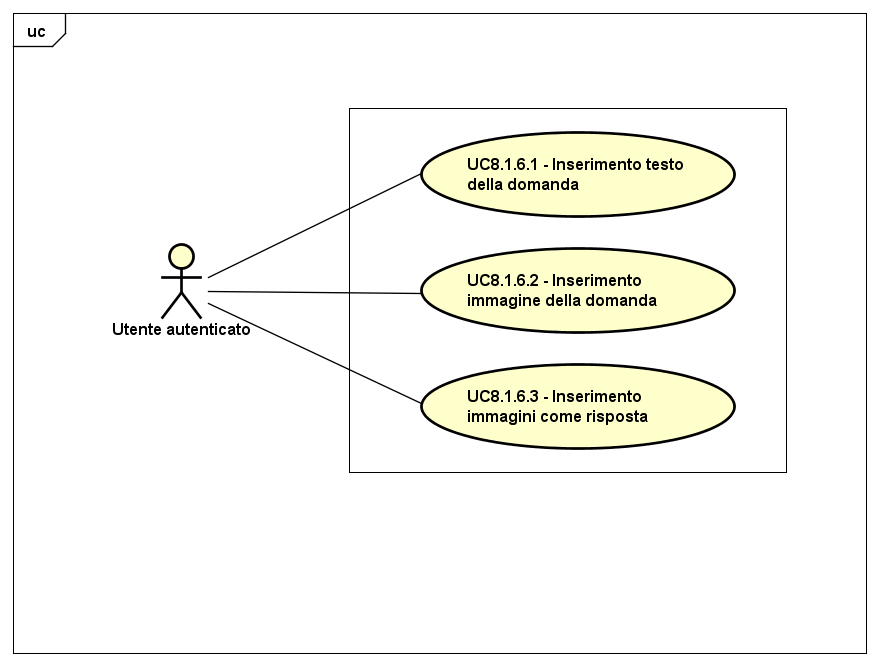
\includegraphics[scale=0.45,keepaspectratio]{UML/UC8_1_6.png}
		\caption{UC8.1.6: Creazione domanda a ordinamento di immagini}
	\end{figure}
	\FloatBarrier
\begin{itemize}
	\item\textbf{Attori}: utente autenticato, utente autenticato pro;
	\item\textbf{Descrizione}: l'attore può utilizzare la procedura guidata per la creazione di una domanda a ordinamento di immagini;
	\item\textbf{Precondizione}: il sistema presenta all'attore la procedura guidata per la creazione di una domanda a ordinamento di immagini; 
	\item \textbf{Postcondizione}: l'attore ha creato una domanda a ordinamento di immagini;
	\item\textbf{Scenario principale}:
	\begin{itemize}
		\item L'attore può inserire il testo della domanda (UC8.1.6.1);
		\item L'attore può inserire un'immagine relativa al testo della domanda (UC8.1.6.2);
		\item L'attore può inserire le immagini della sequenza che costituirà la risposta (UC8.1.6.3).
	\end{itemize}
\end{itemize}

\subsubsection{Caso d'uso UC8.1.6.1: Inserimento testo della domanda}
\begin{itemize}
	\item\textbf{Attori}: utente autenticato, utente autenticato pro;
	\item\textbf{Descrizione}: l'attore può inserire il testo della domanda;
	\item\textbf{Precondizione}: il sistema presenta all'attore lo spazio destinato all'inserimento del testo della domanda;
	\item \textbf{Postcondizione}: l'attore ha inserito il testo della domanda;
	\item\textbf{Scenario principale}: l'attore inserisce il testo della domanda. 
\end{itemize}

\subsubsection{Caso d'uso UC8.1.6.2: Inserimento immagine della domanda}
\begin{itemize}
	\item\textbf{Attori}: utente autenticato, utente autenticato pro;
	\item\textbf{Descrizione}: l'attore può inserire un'immagine relativa al testo della domanda;
	\item\textbf{Precondizione}: il sistema presenta all'attore la funzionalità di inserire un'immagine;
	\item \textbf{Postcondizione}: l'attore ha inserito un'immagine relativa al testo della domanda;
	\item\textbf{Scenario principale}: l'attore inserisce un'immagine.
\end{itemize}

\subsubsection{Caso d'uso UC8.1.6.3: Inserimento immagini come risposta}
\begin{itemize}
	\item\textbf{Attori}: utente autenticato, utente autenticato pro;
	\item\textbf{Descrizione}: l'attore può inserire le immagini che costituiscono la risposta alla domanda e indicare poi la soluzione di questa mettendole nell'ordine corretto;
	\item\textbf{Precondizione}: il sistema presenta all'attore la funzionalità di inserire due o più immagini come risposta; 
	\item \textbf{Postcondizione}: l'attore ha inserito le immagini che costituiscono la risposta alla domanda e le ha ordinate in base alla soluzione di questa;
	\item\textbf{Scenario principale}: l'attore inserisce una o più immagini come risposta.
\end{itemize}

